\chapter{Technologie}\label{chap:technologie}

Niniejszy rozdział zawiera przegląd oraz krótki opis technologii użytych w~procesie realizacji projektu. Przedstawiono najważniejsze cechy każdej z~nich, pomijając szczegóły, wprowadzając jedynie zarys informacji na temat poszczególnych komponentów, na których budowana była aplikacja. Dokonano również podstawowego wprowadzenia do każdej z~wymienionych technologii, co jest potrzebne do pełnego przedstawienia sposobu ich wykorzystania.

\section{Język C\# i platforma .NET}\label{sec:cs}
Język C\# oraz .NET zostały pierwszy raz przedstawione podczas międzynarodowej konferencji dla programistów o nazwie \emph{Professional Developers Conderence} (\acronym{PDC}) w lipcu roku 2000~\cite{ms:initDotNet} - choć środowisko programistów słyszało o planach firmy Microsoft znacznie wcześniej, jednakże pod różnymi nazwami (m.in. COOL, COM3, Lightning). Pomimo sporego w owym czasie szumu wokół niedoskonałych systemów operacyjnych (np. Windows Me), czy też sporych opóźnień w dostarczaniu owych rozwiązań, firma zdecydowała się na stworzenie własnej platformy programistycznej~\cite{cSharp:inDepthF}.

Należy również podkreślić, że firma Microsoft nie była jedyną, która wspierała tworzenie języka - oprócz niej w sponsoring tego języka włączył się firmy Helwett-Packard oraz Intel. Język C\# jest, podobnie, jak język Java, otwartym językiem, jednakże w zupełnie innym tego słowa znaczeniu. Microsoft sprzyja ścieżce standaryzacyjnej języka, gdy Sun (firma posiadająca prawa do platformy Java) stopniowo udostępnia kod źródłowy Javy na zasadach \emph{wolnego oprogramowania} (\english{open source}) i dopuszczając, a nawet zachęcając do tworzenia innych \emph{środowisk uruchomieniowych} (\english{runtime environments}) Javy. Istnieją alternatywne implementacje CLI oraz C\# (najbardziej znanym jest Mono~\cite{cs:mono}), jednakże należy podkreślić, że nie obejmują one swoją implementacją wszystkiego, co kryje się pod nazwą Microsoft .NET Framework. Ostatecznie język C\# oraz .NET zostały udostępnione w roku 2002, razem z narzędziem programistycznym Visual Studio .NET 2002.

\subsection{Platforma .NET}
Kiedy wprowadzono termin ''.NET'', został on wcielony w szereg różnych technologii wychodzących spod sztandarów firmy Microsoft. Na przykład Windows Live ID był nazywany .NET Passport, pomimo tego, że nie istniało żadne bezpoźrednie połączenie pomiędzy tą technologią, a tym co jest obecnie znane, jako .NET. Na całe szczeście z czasem zaprzestano używania nazwy .NET w innych usługach i produktach firmy z Redmond. W chwili obecnej nazwa ''.NET'' wiąże się jedynie ze światem programowania.

Należy podkreślić, że .NET zawiera wspólną specyfikację języka (\acronym{CLS}, \english{Common Language Specification}), która udostępnia zestaw podstawowych reguł, niezbędnch do integracji języków na jednej platformie. CLS określa minimalne wymagania, jakie musi spełniać język z rodziny .NET. Kompilatory zgodne z CLS tworzą obiekty, które mogą ze sobą współpracować.

Poniżej przedstawione zostaną trzy składniki, z jakich zbudowana jest platforma .NET oraz łączące je zależności.

\subsubsection{Język, środowisko uruchomieniowe i biblioteki}
W skład platformy .NET wchodzą trzy podstawowe składniki: język programowania, biblioteki oraz środowisko uruchomieniowe. Wprawdzie rozróżnienie tych trzech nie zawsze jest możliwe, to ważna jest świadomość istnienia wyraźnych różnic pomiędzy tymi trzema składnikami.

\paragraph{Język}
Język C\# jest zdefiniowany przez swoją specyfikację (patrz~\cite{cSharp:spec}), która opisuje format kodu programu w C\#, obejmując jednocześnie składnię oraz zachowanie. Nie jest tam zawarta natomiast informacja o platformie, na jakiej zostanie on uruchomiony, poza kilkoma kilkoma aspektami współpracy kompilatora z platformą. 

W teorii dowolna platforma, która wspiera wymagane funkcje (opisane w specyfikacji), może posiadać kompilator, który będzie budował oprogramowanie przeznaczone dla danej platformy.  Na przykład, kompilator języka C\# mógłby produkować na podstawie kodu źródłowego dowolny inny format niż tzw. \emph{język pośredni} (\acronym{IL}, \english{Intermediate Language}).

\paragraph{Środowisko uruchomieniowe}
Środowisko uruchomieniowe jest częścią .NET odpowiedzialną za dokonanie wszystkiego, by uruchomiony kod IL działał zgodnie ze specyfikacją jęzka. W implementacji firmy Microsoft srodowisko uruchomieniowe nazywa się \emph{Common Language Runtime}, czyli w skrócie \acronym{CLR}.

\paragraph{Biblioteki}
\emph{Biblioteki} (\english{libraries}) dostarczają kod, który może być wykorzystywany przez oprogramowanie. Większość bibliotek frameworka .NET są gotowymi produktami języka IL (patrz punkt~\ref{sec:msil}) z \emph{kodem natywnym} (\english{native code}) wykorzystywanym tylko wtedy, gdy jest to potrzebne. Należy podkreślić, że kodu bilbiotek jest znacznie więcej niż kodu środowiska uruchomieniowego. W taki sam sposób można spojrzeć na samochód (biblioteki), który jest znacznie bardziej skomplikowaną jednostką niż sam jego silnik (środowisko uruchomieniowe).

Warto podkreślić, że istnieje podział na biblioteki standardowe oraz pozostałe, które nie zostały ujęte w specyfikacji języka~\cite{cSharp:spec}. Pisząc program, który wykorzystuje tylko te pierwsze można mieć dużą pewność, że będzie on możliwy do uruchomienia na dowolnej implementacji platformy - czy to Mono, .NET, czy jakiejkolwiek innej.

Termin \emph{.NET} odnosi się do kombinacji środowiska uruchomieniowego wraz z bibliotekami dostarczanymi przez Microsoft, a także kompilatory C\# oraz VB.NET. .NET moze być pojmowany, jako cała \emph{platforma programistyczna} (\english{development platform}) zbudowana nad systemem Windows.


\subsection{Kompilacja i język MSIL}\label{sec:msil}
Programy pisane na platformie .NET nie są kompilowane do plików wykonywalnych, jak to ma miejsce w przypadku chociażby języka C++. Są one kompilowane do podzespołów, które składają się z instrukcji standardowego \emph{języka pośredniego Microsoft} (\acronym{MSIL}, \english{Microsoft Intermediate Language}). Środowisko CLR dokonuje przekształcenia instrukcji tego języka na kod maszynowy i wykonuje je. Pliki MSIL (często zamiennie używa się skrótowej nazwy IL) stworzone przez kompilator języka C\# są niemalże takie same, jak pliki IL innych języków z rodziny .NET. Kluczową cechą środowiska CLR jest to, że jest ono wspólne, co oznacza, że programy napisne w języku VB.NET czy też C\# są obsługiwane przez te samo środowisko uruchomieniowe.

Kompilacja kodu w języku C\# do IL odbywa się w momencie budowania projektu. W wyniku czego kod IL jest zapisywany na dysku w postaci plików binarnych. W momencie uruchomienia programu zachodzi ponowna kompilacja - tym razem kodu IL. Jest to tak zwana kompilacja \acronym{JIT} (\english{Just In Time}), w wyniku której powstaje kod maszynowy, wykonywany przez procesor maszyny, na której program został uruchomiony.

Kompilatory JIT, standardowo, są uruchamiana \emph{na żądanie} (\english{on demand}) - tzn. w momencie wywołania metody, kompilator JIT analizuje kod IL i tworzy bardzo wydajny (dzięki licznym optymalizacjom dokonywanym na tym etapie) kod maszynowy. Gdy aplikacja jest uruchomiona, kompilacja zachodzi jedynie wtedy, kiedy jest to potrzebne, a po kompilacji JIT kod znajduje się w pamięci podręcznej, przez co możliwe jest jego szybkie wykorzystywanie w późniejszych etapach przetwarzania. Wynika z tego, że aplikacja działa tym szybciej, im dłużej jest uruchomiona, ponieważ możliwe jest wykorzystanie większej ilości skompilowanego kodu.

Specyfikacja CLS wymusza podobieństwo kodu IL w przypadku każdego języka z rodziny .NET. Wynika z tego bezpośrednio, że obiekty utworzone w jednym języku mogą być wykorzystywane w programach napisanych w innych językach (z rodziny .NET oczywisćie). Oznacza to np. fakt, że możliwe jest przygotowanie klasy bazowej w języku VB.NET oraz utworzenie od niej klas pochodnych w programie napisanej w języku C\#.

\subsection{Język programowania C\#}
Język C\# jest niezwykle wydajnym narzędziem do implementacji współczesnych technik programistyznych. Jest on językiem obsługującym strukturalne, oparte na komponentach i obiektowe programowanie, czego należy oczekiwać od współczesnego języka, zbudowanego na doświadczeniach z C++ oraz Java. 

Programiści mówiący o nowej wersji .NET, mają zazwyczaj na myśli ważne wydania fremework'a. W większości przypadków wydanie nowej wersji platrofmy jest połączone z wydaniem Visual Studio, czyli zintegrowanego środowiska programistycznego firmy Microsoft. W tabeli~\ref{dotNet:dates} zebrane zostały informacje o poszczególnych wersjach, które były wydawane wraz z jakimi komponentami oraz kiedy.

\begin{table}
	\centering
	\begin{tabular}{l|l|l|l|l}
	\textbf{Data} & \textbf{Framework} & \textbf{Visual Studio} & \textbf{C\#} & \textbf{CLR} \\ \hline
	Luty 2002 & $1.0$ & 2002 & $1.0$ & $1.0$ \\ 
	Kwiecień 2003 & $1.1$ & 2003 & $1.2$ & $1.1$ \\ 
	Listopad 2005 & $2.0$ & 2005 & $2.0$ & $2.0$ \\ 
	Listopad 2006 & $3.0$ & (rozszerzenia do wersji 2005) & [brak] & $2.0$ \\ 
	Listopad 2007 & $3.5$ & 2008 & $3.0$ & $2.0$ SP1 \\ 
	Kwiecień 2010 & $4.0$ & 2010 & $4.0$ & $4.0$ \\
	\end{tabular}
	\caption{Poszczególne wersje .NET Framework oraz ich składniki~\cite{cSharp:inDepthS}\label{dotNet:dates}}
\end{table}

\paragraph{Obiektowość}
\definicja{Programowanie obiektowe} (\akronim{OOP}, \english{Object Oriented Programming}) jest to paradygmat programowania, w~którym program definiuje się przy pomocy obiektów.
Podstawowe cechy języka, który realizuje paradygmat programowania obiektowego przedstawił Alan Kay w~odniesieniu do języka \definicja{Smalltalk}, pierwszego poprawnie zrealizowanego języka obiektowego, a~tym samym jednego z~poprzedników C\#. Cechy te opisują czyste podejście obiektowe.
\begin{description}
	\item \emph{Wszystko jest obiektem.} Obiekt można przedstawić jako specjalną zmienną, która nie tylko zawiera dane, ale może również realizować żądania, czyli wykonywać na swoich danych pewne ściśle określone operacje. Teoretycznie każdy element świata rzeczywistego, np. samochód, dom, zamek, pracownik, może być reprezentowany w~programie przy pomocy tak skonstruowanego obiektu.
	\item \emph{Aplikacja jest zbiorem komunikujących się między sobą obiektów.} Przesyłanie komunikatów do obiektu to żądanie od niego wykonania pewnej operacji. Można to nazwać wykonaniem funkcji należącej do konkretnego obiektu. Przykładem może być następujący scenariusz: obiekt \emph{Kierowca} wysyła do obiektu \emph{Samochód} komunikat \emph{przyspiesz}, co powoduję wykonanie operacji zwiększenia prędkości.
	\item \emph{Każdy obiekt posiada własną pamięć, na którą składają się inne obiekty.} Tworzenie nowego obiektu polega na łączeniu w~jeden element grupy już istniejących obiektów. Powstaje w~ten sposób wielowarstwowa aplikacja, która jednocześnie ukrywa swoją złożoność za prostymi obiektami. Przykładowo obiekt \emph{Samochód} można zbudować z~następujących obiektów: \emph{Karoseria}, \emph{Koło}, \emph{Silnik} itd. Jednocześnie chcąc zwiększyć prędkość pojazdu odwołujemy się do obiektu \emph{Samochód}, a~nie bezpośrednio do obiektu \emph{Silnik}, który odpowiada za jego prędkość. Dopiero akcja \emph{przyspiesz} wykonana przez obiekt Samochód wykonuje odpowiednie operacje na poszczególnych podzespołach, z których się składa.
	\item \emph{Każdy obiekt posiada swój typ.} W~odniesieniu do obiektu słowo \emph{typ} można zastąpić słowem \definicja{klasa}. Każdy obiekt jest instancją pewnej klasy, której głównym zadaniem jest zdefiniowanie jakie komunikaty można wysłać do obiektu będącego jej egzemplarzem.
	\item \emph{Wszystkie obiekty danego typu obsługują te same komunikaty.} Każdy obiekt danej klasy obsługuje wszystkie komunikaty zdefiniowane w~klasie. Dodatkowo jeśli np. obiekt typu \emph{Student} jest jednocześnie obiektem typu \emph{Człowiek}, to obsługuje wszystkie komunikaty zdefiniowane dla typu \emph{Człowiek}. Umożliwia to pisanie bardziej uniwersalnego kodu, który będzie obsługiwał wszystkie obiekty pasujące do typu \emph{Człowiek}~\cite{cSharp:progr}.
\end{description}

Współcześnie, aby język programowania został uznany za obiektowy musi charakteryzować się wymienionymi poniżej cechami.
\begin{description}
	\item[Abstrakcja] Każdy obiekt systemu jest widziany jako abstrakcyjny ,,wykonawca'', który może realizować pracę, określać i~zmieniać swój stan oraz wysyłać komunikaty do innych obiektów w~systemie. Jednocześnie nie ujawnia on jak zostały zaimplementowane dane cechy.
	\item[Hermetyzacja] Czyli ukrywanie wewnętrznej implementacji obiektu. Gwarantuje to, że obiekt nie ma możliwości zmiany stanu wewnętrznego innego obiektu w~nieprzewidziany przez programistę sposób. Tylko metody (funkcje) składowe obiektu mają prawo do modyfikacji jego stanu. Dodatkowo pozwala to na swobodną modyfikację kodu przez programistę o~ile nie zmieniają się metody składowe. Przykładowo w~pierwszej wersji klasy programista może zaimplementować listę jako tablicę o~stałym rozmiarze, natomiast w~kolejnej wersji zmienić tablicę na listę jednokierunkową.
	\item[Polimorfizm] Referencje mogą wskazywać na obiekty różnego, ale zgodnego typu. Wywołanie metody dla referencji spowoduje wykonanie operacji odpowiedniej dla pełnego typu obiektu wywoływanego. Jeśli ma to miejsce w~trakcie działania programu, nazywa się to późnym wiązaniem lub wiązaniem dynamicznym.
	\item[Dziedziczenie] Umożliwia definiowanie specjalizowanych obiektów na podstawie ich ogólniejszych odpowiedników. Podczas definiowania obiektów specjalizowanych nie jest wymagana redefinicja całej funkcjonalności obiektu bazowego, ale tylko ta, której brakuje w~obiekcie ogólniejszym, lub ta, której sposób działania chcemy zmienić.
	
\end{description}

\subsection{Zapytania do obiektów czyli LINQ\label{sec:linq}}
Language INtegrated Query (\acronym{LINQ}) stanowi część technologii frameworka .NET, zaprojektowany i opracowany przez Andersa Hejlsberga, który jest znany z zaprojektowania języka Delphi oraz C\#. Technologia LINQ stworzona została w celu uproszczenia wykonywania zapytań na obiektach, a jego składnia przypomina SQL, przez co jest prostym narzędziem możliwym do wykorzystania przez programistów.

W świecie języków kompilowanych LINQ wydaje się być elementem nie pasującym do standardów, szczególnie przykładowe zapytanie poniżej przypomina bardziej SQL niż język programowania C\#. 

\begin{lstlisting}
var adultNames = from person in people
							where person.Age >= 18
							select person.Name;
\end{lstlisting}

Jednym z powodów, dla których oba języki wyglądają inaczej jest fakt, że LINQ jest \emph{deklaratywny}, a nie \emph{imperatywny} - zapytanie LINQ pyta o pewne właściwości obiektów, zamiast przedstawiać dokładne kroki do osiągnięcia celu. Takie podejście bliskie jest funkcjonalnemu podejściu do rozwiązywania problemów. Co ważne LINQ nie jest przeznaczone jedynie do zapytań wydawanych do baz danych - może ono być bowiem wykorzystywane w operacjach przeprowadzanych w pamięci operacyjnej, na obiektach programu. Dzięki temu właśnie LINQ zdobyło sobie rzesze wiernych użytkowników, którzy na codzień korzystają z dobrodziejstw tego nowoczesnego narzędzia programistycznego.

LINQ został wprowadzony do języka C\# w wersji 3. Celem pracy nie jest opis tej technologii, ale ponieważ stanowiła ona jedną z częściej wykorzystanych została krótko wprowadzona. Po więcej szczegółów należy sięgnąć po~\cite{cSharp:inDepthS}, bądź poświeconą tylko tej technologii książkę~\cite{cSharp:linq}.

\subsection{Kwantyfikator as parallel czyli Parallel LINQ}\label{sec:asparallel}
W opisach procedur znajdowania zbiorów częstych używany jest kwantyfikator \textbf{as parallel}, który jest głównym elementem opisywanego algorytmu ParallelApriori. 

W implementacji algorytmu Apriori technologia LINQ była jedną z częściej wykorzystywanych na obiektach. W roku 2006 Joe Duffy zapowiedział na swoim blogu wprowadzenie nowej technologii, rozszerzającej możliwości LINQ~\cite{cs:helloplinq}. PLINQ (lub też Parallel LINQ) zostało włączone w skład .NET 4, pozwalając budować programy równoległe w bardziej abstrakcyjny sposób. 

Głównym założeniem PLINQ jest fakt, że biorąc wyrażenie LINQ, które wykonywane jest w stosunkowo długim czasie, można zapewnić szybsze jego wykonanie poprzez użycie wielu \emph{wątków} (\english{threads}), które wykorzystają możliwości wielu rdzeni na komputerze - z jak najmniejszą liczbą zmian w kodzie, jak to jest tylko możliwe. Jak w przypadku innych kwestii związanych z programowaniem równoległym - nie jest to aż tak proste podejście, jednakże nawet zwykła zmiana wyrażeń prowadzi zazwyczaj do przyspieszenia działania aplikacji.

Punktem startu dla przeobrażenia wyrażenia LINQ do jego wersji równoległej jest metoda 

\begin{verbatim}
AsParallel()
\end{verbatim}

Jej zastosowanie przekształca wyrażenie, które zostaje podzielone, a następnie będzie wykonywane w środowisku równoległym. Zastosowanie słowa kluczowego \textbf{as parallel} oznacza, że wyrażenie implementowane w przypadku klasycznego algorytmu Apriori (patrz część~\ref{apriori:section}) w LINQ zostało przekształcone w miarę możliwości do nowej technologii, wprowadzonej w ostatniej wersji frameworka .NET.

\subsection{.NET Framework 4.0}
Wydany w roku 2010 w wersji 4.0 framework platformy stanowi podstawę implementacyjną stworzonego w ramach niniejszej pracy oprogramowania. Aplikacja stworzona została przy pomocy najnowszej wersji, czyli 4.0 w zintegrowanym środowisku programistycznym Visual Studio 2010 Professional. 

W wersji 4.0 rozszerzono wiele funkcji dostępnych we wcześniejszych wersjach - m.in. wprowadzająć PLINQ, czyli równoległe wykonywanie zapytań LINQ (\english{Language-INtegrated Query}), które zostało wykorzystane w jednym z zaimplementowanych w ramach niniejszej pracy algorytmie. Poza tym w implementacji wykorzystano szereg wprowadzonych w 4. wersji usprawnień - m.in. nazywane parametry, czy też parametry opcjonalne w metodach. 

Ponieważ nie jest celem niniejszej pracy opisywanie poszczególnych wersji języka, czy też platformy, pominięte zostały szczegóły odnośnie poszczególnych wersji tejże platformy. Doskonałym źródłem informacji o zmianach w poszczególnych wersjach, a także przyczynach zachodzących zmian jest książka Jona Skeeta~\cite{cSharp:inDepthS}.

\section{CUDA}
W realizacji projektu wykorzystana została uniwersalna architektura procesorów wielordzeniowych, która szerzej została omówiona w rozdziale~\ref{chap:cuda}. Użyto NVIDIA CUDA w wersji 3.0, dostępnej do pobrania pod adresem \url{http://developer.nvidia.com/cuda-toolkit-30-downloads} (zweryfikowana dostępność w dniu \today). Językiem wybranym do implementacji metod optymalizujących algorytm został CUDA C, czyli rozszerzenie języka C.

\subsection{CUDA na platformie .NET}
Jak opisano w części~\ref{sec:cs} językiem, który wykorzystano do napisania aplikacji testowej był C\# uruchamiany na platformie .NET. W nawiązaniu do rozdziału~\ref{chap:cuda}, w którym napisano, że NVIDIA wypuściła rozszerzenie języka C (tzn. CUDA C), w którym pojawiły się instrukcje bezpośrednio związane z uniwersalną architektruą wielowątkową CUDA.

Istnieje możliwość użyciać mechanizmów współpracy kodu zarządzanego i natywnego, jednakże istnieją metody znacznie prostrzego wykorzystania możliwośći GPU do obliczeń. Można wykorzystać specjalną bibliotekę, stworzoną do umożliwienia programistom skorzystania z CUDA C wewnątrz programów zarządzanych.

Aby skorzystać z karty graficznej wewnątrz programu przygotowanego na platformę .NET użyta została biblioteka o nazwie CUDA.NET~\cite{cuda:net}. Sposób wykorzystania CUDA wewnątrz aplikacji na platformę .NET przedstawione są poniżej.

\begin{enumerate}
	\item Aplikacja oraz związana z nią logika biznesowa (np. przygotowanie i wyświetlanie danych) pisana jest w języku platformy .NET - w wypadku programu powiązanego z niniejszą pracą był to C\# w wersji $4.0$.
	\item Funkcje obliczeniowe przygotowywane są w języku CUDA C - jako pliki z rozszerzeniem \emph{.cu}. Jest to zgodnie z konwencją pisania programów na platformę CUDA~\cite{Cuda:PGuide}.
	\item Pliki z punktu poprzedniego powinny być skompilowane przy użyciu kompilatora przygotowanego przez firmę NVIDIA - w wyniku tej operacji powstaną pliki o rozszerzeniu \emph{.cubin}. Poniżej zaprezentowane zostało polecenie dla kompilatora wykorzystywane w budowaniu aplikacji, która stanowi podstawę niniejszej pracy.
		\begin{quote}
			\begin{verbatim}
				> nvcc *.cu --cubin
			\end{verbatim}
		\end{quote}
	\item W aplikacji głównej programu należy dodać referencje do biblioteki CUDA.NET, a następnie dopisać kod pośredniczący, w którym przygotowane zostaną dane, uruchomione zostaną funkcje obliczeniowe na karcie graficznej, a następnie odczytane zostaną wyniki tych obliczeń.
\end{enumerate}

Opisaną powyżej architekturę w sposób schematyczny zaprezentowano na rysunku~\ref{rys:arch_cuda_net}.

\begin{figure}[ht]
\centering
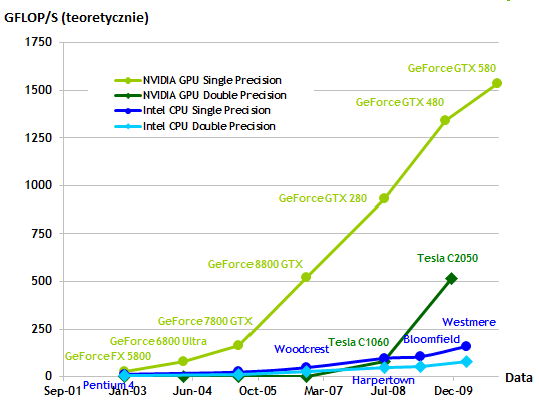
\includegraphics{figures/04/arch_cuda_net.png}
\caption{Schematyczne przedstawienie architektury aplikacji wykorzystującej technologię CUDA przy pomocy biblioteki CUDA.NET}\label{rys:arch_cuda_net}
\end{figure}

\section{Środowisko programistyczne}
W celu ułatwienia pracy podczas przygotowywania aplikacji wykorzystanych został szereg narzędzi ułatwiających prace programiście, a także programistom (w przypadku, gdyby nad projektem pracowała więcej niż jedna osoba). Poniżej krótko opisane zostaną poszczególne narzędzia.

\subsection{Visual Studio 2010}
W pracy nad projektem głównym narzędziem wykorzystywanym do implementacji aplikacji było zintegrowane środowisko programistyczne (\english{Integrated Development Enviroment}, \acronym{IDE}) firmy Microsoft w wersji 2010. Przez IDE rozumie się aplikację (lub ich zespół, czyli środowisko) służącą do tworzenia, modyfikacji, testowania oraz konswerwacji oprogramowania. Programy takie charakteryzują się tym, że udostępniają złożoną, wieloraką funkcjonalność obejmującą edycję kodu źródłowego, kompilowanie kodu źródłowego, tworzenie zasobów programu (tzn. formatek / ekranów / okien dialogowych, menu, raportów, elementów graficznych takich jak ikony, obrazy itp.), tworzenie baz danych, komponentów i innych. Wiele tych funkcji zależy od firmy tworzącej dany program, a także celu wykorzystania danego narzedzia.

Visual Studio~\cite{ms:visualStudio} jest wyżywane do tworzenia różnego rodzaju oprogramowania na platformie .NET, na różnego rodzaju platformy: Microsoft Windows, Windows Mobile, Windows CE, Microsoft Silverlight.

Wykorzystywaną wersą było Microsoft Visual Studio 2010 Ultimate, czyli najwyższa dostępna wersja narzędzia dostępna dla studentów w ramach programu MSDNAA. Samo narzędzie zostało rozszerzone kilkoma dodatkami, o których przeczytać można w kolejnych punktach.

\subsection{System kontroli wersji}
W celu zarządzania kodem wykorzystany został rozproszony system kontroli wersji o nazwie \emph{GIT}. Stworzył go Linus Torvalds, jako narzędzie wspomagające rozwój jądra systemu operacyjnego Linux. Git jest opublikowany na licencji GNU GPL v2, przez co stanowi wolne oprogramowanie z ogólno dostępnym kodem źródłowym. Pierwsza wersja narzędzia Git została wydana 7 kwietnia 2005 roku, kiedy to zastąpiła używany wcześniej w rozwoju Linuksa system kontroli wersji BitKeeper, który w owym czasie zaprzestał darmowe wspieranie oplikacji tworzonych na zasadach wolnego oprogramowania.

Każdy katalog Gita jest pełnoprawnym repozytorium z kompletną historią oraz pełną bazą rewizji wstecznych, niezależnym od dostępu do sieci, czy też centralnego serwera. Dzięki takiemu rozwiązaniu programista jest niezależny od jakichkolwiek awarii, czy też centralnego serwera. 

W tworzeniu aplikacji wykorzystano lustrzany serwer gita utworzony na serwerze GitHub~\cite{cs:github}, będącym uzupełnieniem oraz rezerwą w wypadku awarii głównego repozytorium, zlokalizowanego na komputerze developera, a jednocześnie autora niniejszej pracy.

\subsection{Budowanie projektu}
Ponieważ w tworzeniu aplikacji wykorzystanych zostało kilka różnych technologii (o czym można było przeczytać w poprzednich rozdziałach) zdecydowano, że należy utworzyć jeden sposób do budowania aplikacji oraz zależności pomiedzy poszczególnymi modułami programu. Wykorzystanie samego Visual Studio pozostawało niewystarczające ze względu na wykorzystywaną technologię CUDA.NET, w ramach której należało kompilować pliki .cu, czyli źródła funkcji wykonywanych na karcie graficznej.

Z tychże powodów zdecydowano się wykorzystać psake~\cite{cs:psake}, czyli narzędzie do automatycznego budowania projektu napisane w PowerShell~\cite{ms:powershell}. Poprzez wykorzystywanie w skryptach funkcji oraz stylu wykorzystywanego w PowerShell ułatwia przygotowanie odpowiednich skryptów programiście przeznaczonych do wykorzystania w budowie projektu.

\section{Testowanie}
W ramach projektu wykorzystane zostały \emph{testy jednostkowe} (\emph{unit testing}), które miały zagwarantować poprawność pojedynczych części składowych systemu - np. metod, bądź obiektów, procedur, funkcji. Testowany fragment poddawany jest weryfikacji przez test, który wykonuje go i porównuje wynik (np. zwróconą wartość, stan obiektu, rzucone wyjątki) z oczekiwanymi wartościami - zarówno pozytywnymi, jak i negatywnymi (często testuje się odpowiednie zachowanie programu dla niepoprawnych danych). 

Podstawową zaletą testów jednostkowych jest możliwość ich wykonywania na bieżąco na modyfikowanych elementach programu, co często umożliwia wychwycenie błędu natychmiast po jego pojawieniu się w kodzie programu oraz szybką jego lokalizację, zanim dojdzie do wprowadzenia błędnego fragmentu do ostatecznego kodu programu. Testy jednostkowe są również formą specyfikacji, ponieważ poszczególne metody muszą spełniać odpowiednie założenia. 

\subsection{Usprawnienie procesu testowania}
W ramach twórzenia testów dla projektu wykorzystane zostały nowe narzędzia dostarczone przez firmę Microsoft, które jeszcze bardziej ułatwiają i usprawniają tworzenie aplikacji.

\subsubsection{Code Contracts}
Code Contracts~\cite{ms:codecontracts} są jednym z najnowszych rozszerzeń platformy .NET przygotowane przez Microsoft Research, czyli jednostkę badań i rozwoju dla produktów firmy Microsoft. Code Contracts dostarczają metody wyrażenia założeń wobec metod (oraz innych elementów) w programach na platformie .NET. Kontrakty posiadają formy warunków wejściowych (\english{preconditions}), wyjściowych (\english{postconditions}) oraz ciągłych (\english{object invariants}). Zachowują się one (kontrakty), jak dodatkowa dokumentacja dla wewnętrznego oraz zewnętrznego API aplikacji - tj. dostarczają dodatkowych informacji o metodach wewnątrz projektu. Kontrakty są wykorzystywane do udoskonalenia procesu testowania poprzez weryfikację na poziomie uruchomieniowym (\english{runtime checking}), umożliwiają statyczną weryfikację kontraktu, a także poprzez generowanie dokumentacji kodu, która posiada dodatkowe informacje o metodach - dokumentacja nie bazuje jedynie na informacjach dostarczonych i napisanych przez autora projektu, a także poszczególnych kontraktach na i wewnątrz metod.

Biblioteka Code Contracts wprowadzają do każdego z języków platformy .NET korzyści wynikające z podejścia \emph{projektowanie przez kontrakt} (\english{design-by-contract}). Poniżej wymienione są korzyści wynikające bezpośrednio z wykorzystania Code Contracts.

\begin{itemize}
	\item \textbf{Udoskonalone testowanie}
		\begin{itemize}
			\item Każdy z kontraktów działa na zasadzie wyroczni (\english{oracle}), która powoduje przejście lub nie danego testu.
			\item Automatyczne narzędzia testowania (takie jak Pex, opisany w rozdziale~\ref{04:pex}) mogą wykorzystać wiedzę dostarczoną przez kontrakty do wygenerowania bardziej dokładnych testów jednostkowych, poprzez odfiltrowanie argumentów wejściowych, które nie spełniają warunków wejścia.
		\end{itemize}
	\item \textbf{Statyczna weryfikacja}
		Microsoft przygotował zestaw narzędzi do statycznej weryfikacji kodu, dostarczając informacji o możliwych niedoskonałościach oprogramowania. Obecnie narzędzie może wykorzystać kontrakty do dostarczenia większej ilości i bardziej dokładnych informacji na temat błędów w programie.
	\item \textbf{Dokumentacja API}
		Dokumentacja API projektu często jest niepełna, bądź niewystarczająca. Te same kontrakty, które wykorzystywane są do testowania podczas uruchomienia, a także do statycznej weryfikacji mogą być również wykorzystane do wygenerowania lepszej dokumentacji projektu, np. poprzez dostarczenie informacji o tym, które parametry wejściowe nie mogą mieć wartości \emph{null}.
\end{itemize}

Wykorzystanie biblioteki pozwala praktycznie każdemu językowi z platformy .NET skorzystać z możliwości, jakie niosą ze sobą kontrakty wewnątrz kodu aplikacji. Nie ma potrzeby pisania parsera, czy też kompilatora (lub dodatków do niego) języka. Co więcej, odpowiednie kompilatory języków w naturalny sposób dokonują weryfikacji poprawności poszczególnych kontraktów (sprawdzanie typów oraz nazw), a także produkują skompilowane formy kontraktów w języku MSIL. Tworzenie kontraktów w Visual Studio pozwala programiście skorzystać dodatkowo z możliwości \emph{podpowiedzi} (\english{intelisense}) dostarczanych przez serwisy języka. Poprzednie podejścia poprzez zastosowanie atrybutów .NET przegrywają z tym podejściem, ponieważ nie mogły w wystarczający sposób być wykorzystane w bardziej skompikowanych kontraktach, a także nie mogły one być wykorzystane w trakcie weryfikacji podczas kompilacji.

Kontrakty są wyrażone poprzez wywołania statycznych metod na początku metody. Narzędzia projektu biorą odpowiedzialność za interpretację zadeklarowanych kontraktów w odpowiednich miejscach programu. Biblioteka Code Contracts jest zlokalizowana w przestrzeni nazw \emph{System.Diagnostics.Contracts} platformy w wersji $4.0$.

\subsubsection{Pex i Moles\label{04:pex}}
Pex jest narzędziem rozszerzającym możliwości Visual Studio 2010 w kwestii testów jednostkowych na aplikacjach platformy .NET. Pex tworzy zestaw \emph{testów białej skrzynki} (\english{white box testing}), zwanych również testami strukturalnymi lub szklanej skrzynki. Testy takie polegają na poddaniu programu testowaniu poprzez podawanie na wejściu takich danych, by program przeszedł przez każdą ścieżkę wykonania programu. Zasady przejścia definiowane są przez kryteria pokrycia wszystkich pętli oraz wszystkich warunków w programie (metodzie programu). Testy białej skrzynki nie są w stanie wykazać braku implementacji finkcji, którą powinien posiadać docelowy produkt. Testy te dokonują sprawdzenia operacji wykonywanych wewnątrz zaimplementowanych metod. 

Co ważne Pex wykorzystuje informacje dostarczane przez Code Contracts, co pozwala temu narzędziu wygenerowanie bardziej dokładnych testów dla poszczególnych metod. Testy generowane są automatycznie, jednocześnie zapewniają one wysoki stopień pokrycia kodu testami. Istnieje również możliwość wygenerowania małych zestawów danych prosto z edytora Visual Studio i zachowania ich, jako małe zestawy testów z wysokim stopniem pokrycia (dla danej metody, czy też klasy).

Pex dostarczany jest w zestawie z Moles. Biblioteka ta umożliwia zastąpienie każdej metody w programie dowolnym delegatem. Dzięki temu możliwe jest wyizolowanie kodu z zewnętrznych zależności, w celu przetestowania działania kodu zgodnie z intencją programisty. Moles automatycznie generuje odpowiednie delegaty dla każdej zależności wobec zewnętrznej biblioteki.